\documentclass[../proyecto.tex]{subfiles}

\begin{document}
\chapter{Implementación}

\section{Sensor}

Como se ha comentado en el análisis de tecnologías para la realización de este sensor se ha seleccionado el SoC ESP32, utilizando una placa de desarrollo ESP32 DevKitC de Espressif y para el desarrollo del código se ha elegido el \textit{framework} Arduino aunque para algunas funcionalidades de más bajo nivel se utilizarán librerías del \textit{framework} ESP-IDF.\\

Para la estructuración del código principal se ha utilizado la estructura básica de \textit{Sketch} de Arduino consistente en dos fases: \textit{Setup} y \textit{Loop}. La fase de \textit{Setup} solo se ejecutará una vez en cada encendido o reinicio del dispositivo y en ella se realizan las tareas de incialización del dispositivo. Una vez realizada la inicialización se ejecutará la fase \textit{Loop}, se trata de un bucle infinito en el que se definirá la lógica del sensor.\\

Durante la fase de inicialización el módulo ejecutará secuencialmente las siguientes tareas:
\begin{itemize}
  \item Generar identificador único utilizado para enviar las detecciones al servidor central.
  \item Conéctar a una red WiFi para sincronizar la hora mediante el prótocolo SNTP.
  \item Inicializar el escaneo Bluetooth.
  \item Inicializar el escaneo WiFi.
\end{itemize}

A continuación se realizará una breve descripción del código relacionado con la detección de las tramas Bluetooth y WiFi, y del procedimiento para su envío al servidor central.\\

Para realizar la detección de dispositivos Bluetooth se ha utilizado la librería \textit{BLEScan} incluida en las librerías de Arduino para el ESP32, esta librería crea una capa de abstracción sobre las librerías de BLE de ESP-IDF facilitándonos una API que se adapta a la mayoría de casos de uso al mismo tiempo que provee de métodos para ajustar y adaptar a más bajo nivel para casos más complejos.\\

Esta librería reduce enormemente la complejidad del código ya que además de simplificar la interacción con las librerías de \textit{ESP-IDF} nos proporciona otras ventajas como la posibilidad de registrar una función \textit{callback} asíncrona que será invocada cada vez que un dispositivo sea detectado.\\

En la función \textit{callback} se extraerá la dirección Bluetooth del anunciante y se guardará la fecha y hora de la detección en formato de fecha Epoch.\\

\begin{minipage}{\linewidth}
\begin{lstlisting}[language=C++, caption=Función \textit{callback} para el escaneo BLE, captionpos=b, frame=single]
class ble_advertised_device_cb: public BLEAdvertisedDeviceCallbacks {
    void onResult(BLEAdvertisedDevice advertisedDevice) {
        time_t now;
        time(&now);
        String bd_addr = advertisedDevice.getAddress().toString().c_str();
        ble_detected[bd_addr] = now;

        #if DEBUG == 1
        Serial.println();
        struct tm timeinfo;
        localtime_r(&now, &timeinfo);
        Serial.printf("Bluetooth detection: | MAC: %s ", advertisedDevice.getAddress().toString().c_str());
        Serial.print(" - Time: ");
        Serial.print(&timeinfo);
        Serial.println();
        #endif
    }
};Z
\end{lstlisting}
\end{minipage}

Para monitorizar el tráfico WiFi ha sido necesario utilizar funciones de la API de ESP-IDF ya que las librerías de Arduino no proveen la posibilidad de activar el modo promiscuo necesario para poder analizar todo el tráfico WiFi y no solo el dirigido a nuestro dispositivo.\\

La API de \textit{Networking} del ESP-IDF nos permite activar el modo promiscuo en la interfaz WiFi y además permite registrar una función \textit{callback} asíncrona que será invocada cada vez que un paquete es recibido, pero como se observó en el análisis del estándar WiFi para la detección de dispositivos solo necesitamos los paquetes de tipo \textit{management} y por tanto ejecutar el análisis del paquete con cada evento supondría una gran penalización en rendimiento, pero gracias a la función \textit{esp\_wifi\_set\_promiscuous\_filter} podemos establecer un filtro para determinar que tipo de paquetes dispararan la llamada a la función \textit{callback}, en concreto podemos utilizar el filtro \textit{WIFI\_PROMIS\_FILTER\_MASK\_MGMT}.\\

\begin{minipage}{\linewidth}
\begin{lstlisting}[language=C++, caption=Activación del modo promiscuo con filtrado, captionpos=b, frame=single]
const wifi_promiscuous_filter_t filter={.filter_mask=WIFI_PROMIS_FILTER_MASK_MGMT};
esp_wifi_set_promiscuous_filter(&filter);
esp_wifi_set_promiscuous_rx_cb(&Sniffer::sniffer_callback);
esp_wifi_set_promiscuous(true);
\end{lstlisting}
\end{minipage}

Las librerías de ESP-IDF nos proporcionan una estructura de datos para el almacenamiento del paquete recibido por la función \textit{callback} pero en esta estructura solo se define miembros para los metadatos de la capa de radio como el canal dónde se ha recibido el paquete o la fuerza de la señal, sin embargo el propio \textit{frame} se presenta como un simple puntero a los datos en bruto, esta estructura por tanto resulta ineficiente para la manipulación de los campos que necesitamos y es necesario definir nuestras propias estructuras de datos para almacenar la trama IEEE802.11 de tipo \textit{management}.\\

\begin{minipage}{\linewidth}
\begin{lstlisting}[language=C++, caption=Estructuras de datos para almacenamiento de las cabeceras IEEE802.11 , captionpos=b, frame=single]
struct frame_control {
    unsigned protocol_version:2;
    unsigned type:2;
    unsigned subtype:4;
    uint8_t stuff;
} __attribute__((packed));

struct iee80211_header {
    struct frame_control frame_control;
    uint16_t duration_id;
    uint8_t address_1[6];
    uint8_t address_2[6];
    uint8_t address_3[6];
    uint16_t seq_ctrl;
};
\end{lstlisting}
\end{minipage}

Una vez definidas las estructuras de datos necesarias podemos realizar el análisis de la trama en busca de la dirección de la estación emisora, esta lógica se define dentro de la función \textit{callback} descrita anteriormente. En esta función se realizará la extracción de la dirección MAC y se almacenará junto a la fecha y hora de detección en formato de tiempo Epoch.\\

\begin{minipage}{\linewidth}
\begin{lstlisting}[language=C++, caption=Función \textit{callback} para el modo promiscuo , captionpos=b, frame=single]
void ICACHE_FLASH_ATTR Sniffer::sniffer_callback(void *buff, wifi_promiscuous_pkt_type_t type)
{
    if (type == WIFI_PKT_MGMT) { //Maybe unnecessary after filter
        // Obtenemos el
        const wifi_promiscuous_pkt_t *packet = (wifi_promiscuous_pkt_t *)buff;

        struct Sniffer::iee80211_header *header = (struct iee80211_header*) packet->payload;
        if (header->frame_control.type == TYPE_MANAGEMENT
            && header->frame_control.subtype == SUBTYPE_PROBE_REQUEST) {
              time_t now;
              time(&now);
              // The second address in MAC header is the transmitting station.
              uint8_t *addr = header->address_2;
              char mac_addr[18];
              sprintf(mac_addr, "%02x:%02x:%02x:%02x:%02x:%02x", addr[0], addr[1], addr[2], addr[3], addr[4], addr[5]);
              sta_detected[String(mac_addr)] = now;
              #if DEBUG == 1
                Serial.println();
                struct tm timeinfo;
                localtime_r(&now, &timeinfo);
                Serial.print( "WiFi detection | MAC: " + String(mac_addr) );
                Serial.print(" - Time: ");
                Serial.print(&timeinfo);
                Serial.println();
              #endif
        }
    }
}
\end{lstlisting}
\end{minipage}

Una vez lanzados los procesos asíncronos de detección en el bucle principal se comprobará si el número de detecciones realizadas supera el umbral establecido, esta comprobación se realiza en intervalos de 200 ms y una vez alcanzado el umbral la detección se detendrá temporalmente para dar paso al envío de las detecciones al servidor central, la detención del escaneo es necesaria ya que el módulo no puede estar en modo promiscuo y en modo estación simultáneamente. El umbral establecido es de 100 detecciones, este umbral ha sido calculado en base a las limitaciones de memoria del módulo y a minimizar el tiempo de parada que será necesario para el envío de las detecciones.\\

\begin{minipage}{\linewidth}
\begin{lstlisting}[language=C++, caption=Bucle principal , captionpos=b, frame=single]
void loop() {
    uint32_t detecions_count = Sniffer::sta_detected.size() + ble_detected.size();
    if (detecions_count >= 100) {
        p_ble_scan->stop();
        promiscuous_mode(false);
        send_detections();
        p_ble_scan->start(5, scan_complete_cb, false);
        promiscuous_mode(true);
    }
    if (!ble_scan_active) {
        p_ble_scan->start(5, scan_complete_cb, false);
        ble_scan_active = true;
    }
    Sniffer::channel_hop();
    delay(200);
}
\end{lstlisting}
\end{minipage}

La fase de envío de detecciones consiste principalmente en dos fases, en primer lugar se serializan las detecciones en un documento json  y en la segunda fase se envían mediante HTTP al servidor central. Para el envío de las detecciones al servidor central se utilizan la librería HTTPClient incluida en el core de Arduino, esta libería permite realizar fácilmente peticiones GET, POST y PUT a servidores HTTP. También se ha usado la librería ArduinoJson de Benoît Blanchon que permite serializar fácilmente las detecciones en un objeto JSON que se utilizará para el envío al servidor central mediante una petición POST.

\begin{minipage}{\linewidth}
\begin{lstlisting}[language=C++, caption=Envío de detecciones al servidor central , captionpos=b, frame=single]
void send_detections() {
    Serial.println("Sending detections. ");
    connect_wifi();

    // Memory pool for JSON object tree (bytes).
    DynamicJsonDocument json_doc(20000);

    json_doc["node"] = station_id;
    JsonObject detections = json_doc.createNestedObject("detections");
    for (std::map<String,uint32_t>::iterator it=Sniffer::sta_detected.begin(); it!=Sniffer::sta_detected.end(); ++it) {
        detections[md5(it->first)] = it->second;
    }
    for (std::map<String,uint32_t>::iterator it=ble_detected.begin(); it!=ble_detected.end(); ++it) {
        detections[md5(it->first)] = it->second;
    }

    // Clear detecions
    Sniffer::sta_detected.clear();
    ble_detected.clear();

    #if DEBUG == 1
    serializeJsonPretty(json_doc, Serial);
    Serial.println();
    #endif

    String databuf;
    serializeJson(json_doc, databuf);
    // Post detections
    HTTPClient http;
    http.begin(SERVER_URL);
    http.addHeader("Content-Type", "application/json");
    http.POST(databuf);
    http.end();
}
\end{lstlisting}
\end{minipage}

\section{Servidor Central}

Como se comentó en la introducción de este trabajo una de los objetivos secundarios consiste en almacenar y poder visualizar todas las detecciones realizadas por los sensores en un servidor central, con este propósito se ha desarrollado una API REST basada en HTTP, usando JSON como formato de intercambio de datos. Además se ha desarrollado una interfaz web para poder visualizar de una forma más cómoda las detecciones.\\

Para el desarrollo de la API y la interfaz web se ha utilizado el \textit{framework} de desarrollo web Flask, para desplegar está herramienta se han utilizado contenedores

\begin{figure}[H]
\centering
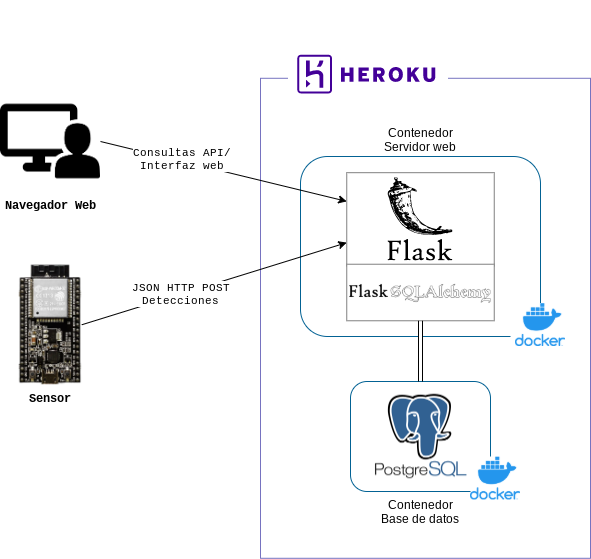
\includegraphics[scale=0.5]{implementacion/estructura_servidor_central}
\caption{Estructura servidor central }
\label{fig:estructura_servidor_central}
\end{figure}


\begin{minipage}{\linewidth}
\begin{lstlisting}[caption=Dockerfile del servidor web, captionpos=b, frame=single]
FROM python:alpine

EXPOSE 5000

ENV VIRTUAL_ENV=/opt/venv

RUN adduser -D vedetra

WORKDIR /home/vedetra

COPY requirements.txt requirements.txt

RUN apk --update add --no-cache --virtual .build-deps \
    gcc \
    musl-dev \
    postgresql-dev \
 && apk --update add --no-cache postgresql-client \
 && python -m venv "$VIRTUAL_ENV" \
 && ${VIRTUAL_ENV}/bin/pip install --no-cache-dir -r requirements.txt \
 && apk del --no-cache .build-deps

USER vedetra

COPY app app
COPY tests tests
COPY migrations migrations
COPY vedetra-server.py config.py  entrypoint.sh ./

ENTRYPOINT ["./entrypoint.sh"]
\end{lstlisting}
\end{minipage}

The Compose file is a YAML file defining services, networks and volumes.

\begin{minipage}{\linewidth}
\begin{lstlisting}[caption=Descripción Docker Compose, captionpos=b, frame=single]
version: '3'
services:
  vedetra:
    build: .
    ports:
      - "5000:5000"
    env_file:
      - web.env.sample
    depends_on:
      - "db"
  db:
    image: "postgres:11-alpine"
    restart: always
    env_file: db.env.sample
    expose:
      - 5432
\end{lstlisting}
\end{minipage}

\begin{minipage}{\linewidth}
\begin{lstlisting}[caption=Definición de aplicación de Heroku, captionpos=b, frame=single]
build:
 docker:
   web: Dockerfile
run:
 web: exec gunicorn vedetra-server:app
\end{lstlisting}
\end{minipage}

Heroku


\end{document}
